\chapter{Von der Teilchenmechanik zu klassischen Feldern}

\section{Was ein Feld ist}

In der vorangegangenen Vorlesung wurde die relativistische Teilchenmechanik ausgehend von einer invarianten Wirkung entwickelt. Nun ändern wir das dynamische Objekt. Gegenstand ist die klassische Feldtheorie, nicht die Quantenfeldtheorie. Die Quantenmechanik wird gelegentlich einen nützlichen Vergleich liefern, doch die Gleichungen in diesem Kapitel beschreiben gewöhnliche klassische Felder. Elektromagnetismus dient als vertrautes Modell im Hintergrund: Elektromagnetische Wellen breiten sich durch den Raum aus und wechselwirken mit geladenen Teilchen. Wir beginnen mit einem noch einfacheren Feld.

Eine Raumzeit kann viele räumliche Koordinaten haben, aber nur eine Zeitkoordinate. Wir schreiben \begin{equation}
x^\mu=(t,x^1,\ldots,x^d),
\end{equation}, wobei der räumliche Index \(i=1,\ldots,d\) gilt. Die Zahl \(d\) kann wie in unserer Welt drei sein, oder eins, zwei, neun, fünfundzwanzig oder eine andere für ein Modell nützliche Zahl. Die entscheidende Asymmetrie besteht hier darin, dass es weiterhin nur eine Zeitrichtung gibt. Die Vorlesung versucht nicht zu erklären, warum Theorien mit mehreren Zeiten so schwierig sind; sie legt einfach den Rahmen mit einer Zeit zugrunde, in dem gewöhnliche kausale Physik formuliert wird.

Ein Feld ist eine messbare Größe, deren Wert sich von Ort zu Ort und von Zeit zu Zeit ändern kann. Ein einfaches Beispiel ist die Temperatur: \begin{equation}
T=T(\mathbf{x},t).
\end{equation} Sie ordnet jedem Ereignis eine Zahl zu und ist daher ein Skalarfeld. Auch die Windgeschwindigkeit variiert mit Ort und Zeit, hat aber Betrag und Richtung und damit mehrere Komponenten; sie ist ein Vektorfeld. In der relativistischen Physik haben die natürlichen Vektoren vier statt drei Komponenten.

Während des größten Teils dieser Vorlesung hat das Feld eine Komponente und wird mit dem griechischen Buchstaben bezeichnet, der \(f\) entspricht: \begin{equation}
\phi=\phi(\mathbf{x},t).
\label{eq:sr4-field-definition}
\end{equation} Dass \(\phi\) ein Skalar heißt, wird schließlich mehr bedeuten, als dass es nur eine Komponente hat. Es bedeutet, dass alle Inertialbeobachter \(\phi\) am selben physikalischen Ereignis denselben Wert zuordnen. Dieses Transformationsgesetz kommt erst ins Spiel, nachdem die Variationsmechanik entwickelt wurde.

\section{Das Teilchen als Vorbild}

\subsection{Eine Koordinate namens \texorpdfstring{\(\phi\)}{phi}}

Der schnellste Weg zur Feldtheorie führt über einen Schritt zurück zu einem gewöhnlichen nichtrelativistischen Teilchen. Das Teilchen bewege sich auf einer Geraden, aber seine Koordinate heiße \(\phi\) statt \(x\). Es gibt keinen mathematischen Grund, eine Koordinate \(x\) zu nennen; der ungewöhnliche Name soll die folgende Analogie sichtbar machen. Tragen wir die Zeit horizontal auf. Dann ist die gesamte Geschichte des Teilchens eine Kurve \(\phi(t)\), die positive wie negative Werte annehmen kann.

Für feste Anfangs- und Endzeiten \(a\) und \(b\) lautet die Wirkung \begin{align}
A[\phi]
&=\int_a^b dt\,L(\phi,\dot\phi),\\
L(\phi,\dot\phi)
&=\frac{m}{2}\dot\phi^{\,2}-V(\phi).
\label{eq:sr4-particle-lagrangian}
\end{align} Die Euler--Lagrange-Gleichung lautet \begin{equation}
\frac{d}{dt}\left(\frac{\partial L}{\partial\dot\phi}\right)
-\frac{\partial L}{\partial\phi}=0.
\label{eq:sr4-particle-el}
\end{equation} Für die Lagrange-Funktion aus \eqref{eq:sr4-particle-lagrangian} gilt \begin{equation}
\frac{\partial L}{\partial\dot\phi}=m\dot\phi,
\qquad
\frac{\partial L}{\partial\phi}=-\frac{dV}{d\phi},
\end{equation}, also \begin{equation}
\boxed{m\ddot\phi=-\frac{dV}{d\phi}}.
\label{eq:sr4-newton}
\end{equation} Das ist einfach die Newton-Gleichung, geschrieben mit \(\phi\) als Koordinate.

\begin{figure}[htbp]\centering
\includegraphics[width=0.90\textwidth]{lecture_04_figure_01.png}\caption{Die gewöhnliche Euler--Lagrange-Gleichung und ihr Newtonsches Ergebnis für die Koordinate \(\phi(t)\).}\lectureframe{00:10:18}\end{figure}

Der physikalische Pfad macht die Wirkung stationär, wenn die Endpunkte festgehalten werden. In der Vorlesung heißt es oft \emph{Minimum}, doch die präzise Aussage lautet Stationarität: Der Pfad kann ein Minimum, ein Maximum oder einen anderen stationären Wert ergeben. Ein nützliches gedankliches Modell besteht darin, das Zeitintervall in viele kleine Stücke zu zerlegen. Die Wirkung wird dann zu einer Funktion der vielen abgetasteten Werte von \(\phi\). Diese Werte zu verändern, während die Endpunkte fest bleiben, und nach jedem einzelnen abzuleiten, ist der endlichdimensionale Vorläufer der Euler--Lagrange-Gleichung.

\subsection{Mechanik als Theorie in \texorpdfstring{\(0+1\)}{0+1} Dimensionen}

Stellen wir uns nun eine Welt mit Zeit, aber ohne räumliche Dimensionen vor. Ihr Raum besteht aus einem einzigen Punkt. Ein Feld in dieser Welt kann nicht vom Ort abhängen, weil es keinen Ort gibt, von dem es abhängen könnte; es kann nur eine Funktion \(\phi(t)\) sein. Die gewöhnliche Mechanik mit einer Koordinate lässt sich daher als Feldtheorie in \(0+1\) Dimensionen auffassen. Die Mathematik hat sich nicht geändert. Nur die Deutung ist eine andere: Statt der Position eines Teilchens betrachten wir nun den Wert eines Feldes in einer Welt ohne Raum.

\begin{figure}[htbp]\centering
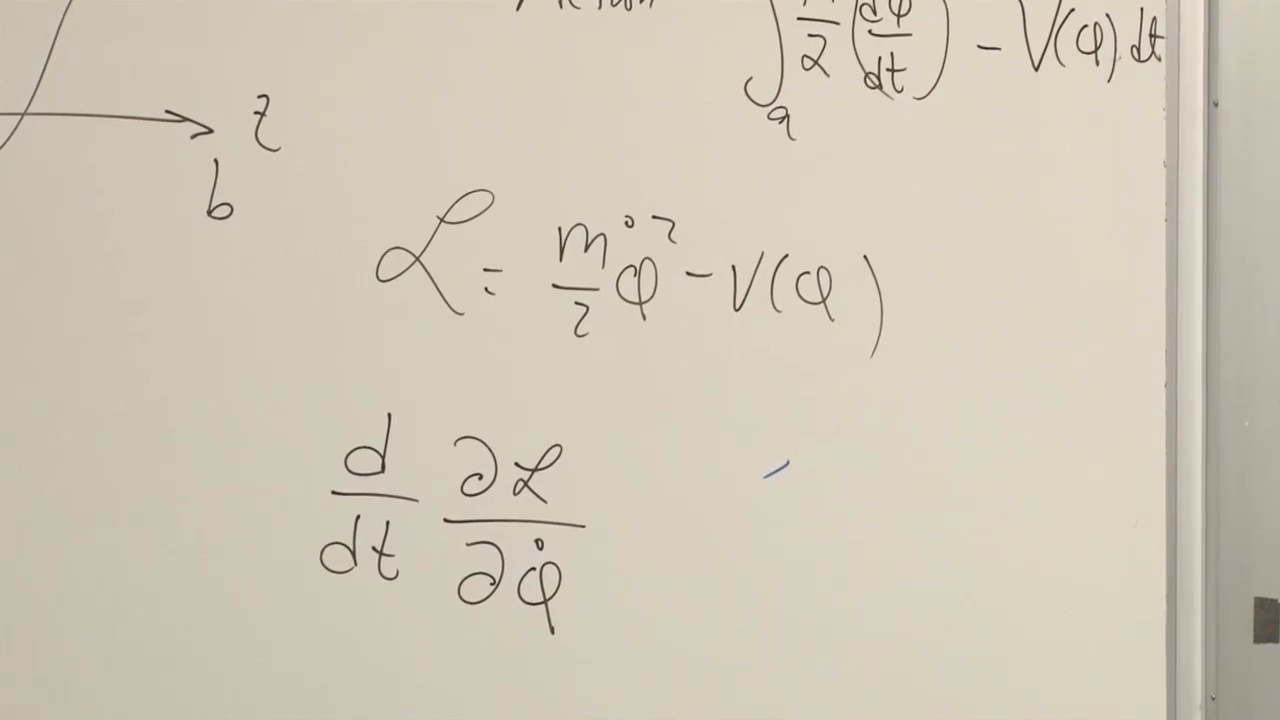
\includegraphics[width=0.90\textwidth]{lecture_04_figure_02.png}\caption{Die abgetastete Geschichte \(\phi(t)\): eine Teilchenbahn und, neu interpretiert, eine Feldgeschichte in \(0+1\) Dimensionen.}\lectureframe{00:14:30}\end{figure}

\begin{classroomqa}\audiencequestion{Verschwindet das Potential, wenn es keine räumlichen Dimensionen gibt?}\lecturerresponse{Nein. Die räumliche Variation verschwindet, aber das Feld hat weiterhin einen Wert. Die Energie kann von diesem Wert über \(V(\phi)\) abhängen. In der Teilchendeutung ändert eine Verschiebung der Kurve nach oben oder unten die potenzielle Energie; in der Felddarstellung tragen verschiedene Werte von \(\phi\) unterschiedliche potenzielle Energie. \lecturetimestamp{00:15:00}}\end{classroomqa}

\begin{classroomqa}\audiencequestion{Kann man sich statt eines Raums ohne Dimensionen auch einen gewöhnlichen Raum vorstellen, in dem das Feld nur von der Zeit abhängt?}\lecturerresponse{Ja. Für diesen Zweck ist die lokale Mathematik dieselbe: Alle räumlichen Ableitungen verschwinden, und nur \(\phi(t)\) bleibt. Die Bezeichnung als Theorie in \(0+1\) Dimensionen hebt diese reduzierte Struktur hervor, aber auch ein räumlich homogenes Feld in einer Welt mit mehr Dimensionen vermittelt dieselbe Anschauung. \lecturetimestamp{00:16:25}}\end{classroomqa}

Der Sinn dieses Umwegs ist nun klar. Wir kennen das Wirkungsprinzip für ein Feld, das von einer Koordinate, der Zeit, abhängt. Das daraus erkennbare Muster können wir nutzen, um das Wirkungsprinzip für ein Feld zu erschließen, das von allen Raumzeitkoordinaten abhängt.

\section{Eine Feldgeschichte über der Raumzeit}

\subsection{Von der Kurve zur Fläche}

In \(1+1\) Dimensionen ist die Raumzeit selbst eine Ebene mit den Koordinaten \(t\) und \(x\). Der Wert \(\phi(x,t)\) liefert eine dritte Richtung. Die Geschichte des Feldes ist daher keine Kurve, sondern eine Fläche über der Raumzeitebene. Die Fläche kann über null ansteigen oder darunter fallen, denn ein Skalarfeld muss nicht positiv sein.

\begin{figure}[htbp]\centering
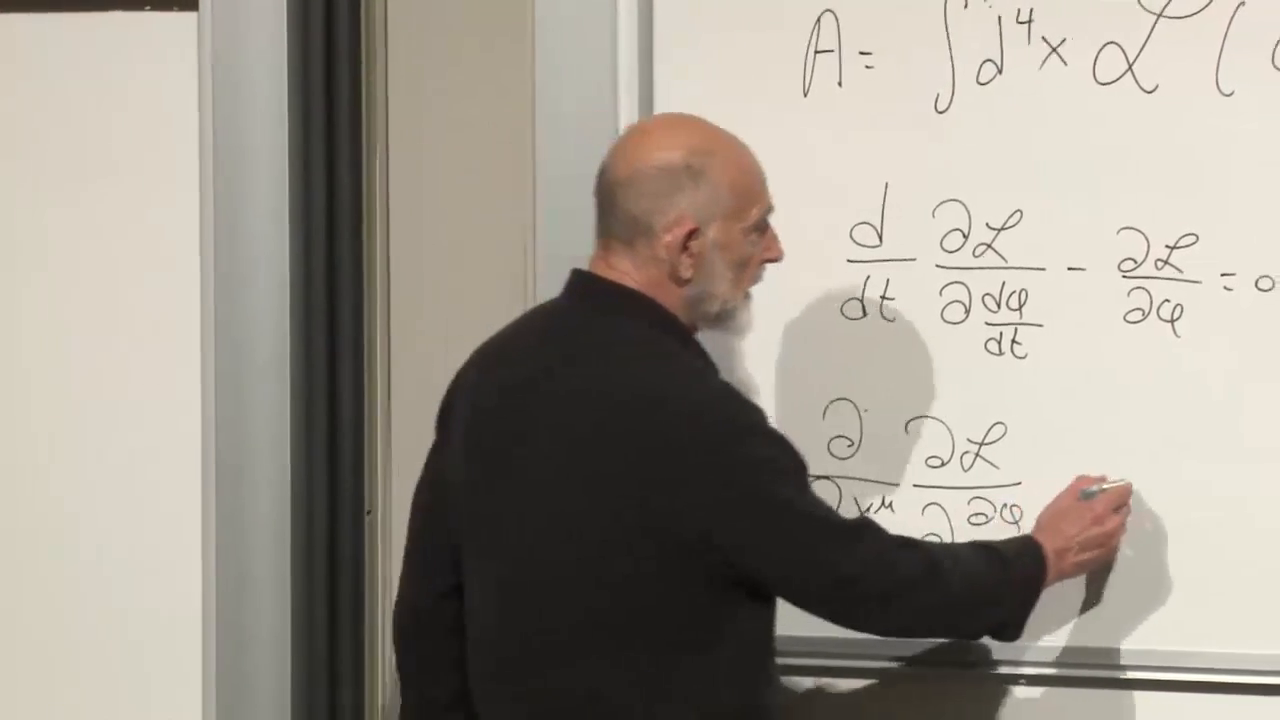
\includegraphics[width=0.90\textwidth]{lecture_04_figure_03.png}\caption{Eine Skalarfeldgeschichte, dargestellt als Fläche über einer Raumzeitebene mit \(1+1\) Dimensionen.}\lectureframe{00:20:46}\end{figure}

Unsere physikalische Raumzeit heißt \(3+1\)-dimensional: Sie hat drei Raumdimensionen und eine Zeitdimension. Ein Modell auf einer Tischplatte ist \(2+1\)-dimensional, und Perlen auf einem Draht veranschaulichen eine Welt mit \(1+1\) Dimensionen. Die zusätzliche Achse, die zur Darstellung von \(\phi\) nötig ist, macht selbst den Fall \(3+1\) unmöglich originalgetreu zeichnbar. Die Definition ist jedoch eindeutig: Eine vollständige Geschichte ordnet jedem Raumzeitereignis einen Wert von \(\phi\) zu.

\subsection{Von festen Endpunkten zu festen Randdaten}

Beim Variationsproblem für ein Teilchen werden zwei Endpunkte festgehalten und die Kurve dazwischen variiert. Das Analogon in der Feldtheorie wählt ein Raumzeitgebiet aus, hält \(\phi\) auf dessen Rand fest und variiert \(\phi\) im Inneren. Das Gebiet kann in einer Zeichnung mit \(1+1\) Dimensionen ein Rechteck sein oder in einer Raumzeit höherer Dimension ein beliebiges geeignetes Gebiet.

\begin{figure}[htbp]\centering
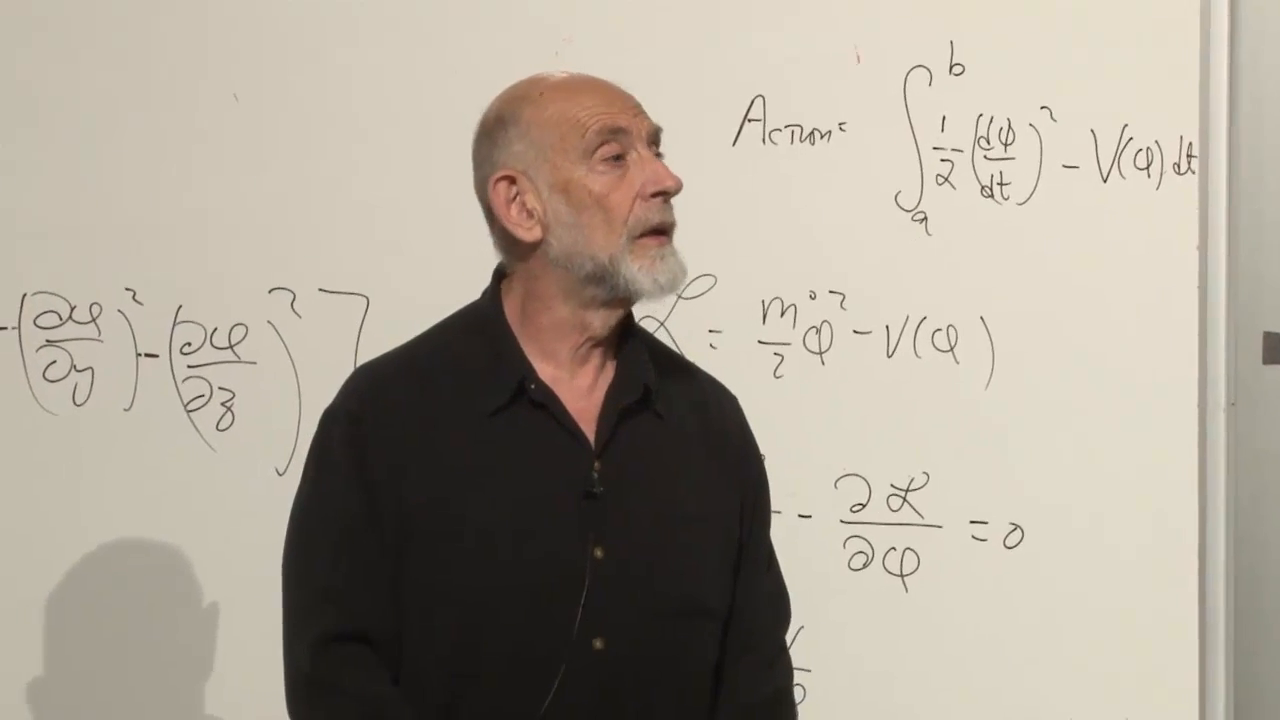
\includegraphics[width=0.90\textwidth]{lecture_04_figure_04.png}\caption{Ein Raumzeitgebiet, dessen gesamter Rand festgehalten wird, während das Feld im Inneren variiert wird.}\lectureframe{00:24:52}\end{figure}

\begin{classroomqa}\audiencequestion{Funktioniert die Lagrange-Formulierung auch dann, wenn ein Potential explizit von der Zeit abhängt?}\lecturerresponse{Ja. Die Euler--Lagrange- und die Hamilton-Formulierung funktionieren weiterhin. Im Allgemeinen geht jedoch die Energieerhaltung verloren: Explizite Zeitabhängigkeit bricht die Zeittranslationssymmetrie. In der Feldtheorie ist die entsprechende Aussage, dass eine explizite Raumzeitabhängigkeit zulässig ist, obwohl sie die zugehörigen Erhaltungssätze beeinflusst. \lecturetimestamp{00:23:49}}\end{classroomqa}

\begin{classroomqa}\audiencequestion{Wird beim rechteckigen Feldgebiet nur der obere und der untere Rand festgehalten oder der ganze Rand?}\lecturerresponse{Bei dieser Variationskonstruktion wird der ganze Rand festgehalten: alle vier Seiten des Rechtecks mit \(1+1\) Dimensionen. Das Feld darf nur im Inneren variieren. Dies ist das direkte Analogon dazu, beide Endpunkte in der Teilchenmechanik festzuhalten. \lecturetimestamp{00:24:24}}\end{classroomqa}

Den gesamten Rand festzuhalten ist eine Festlegung für die Variation, mit der die Gleichungen hergeleitet werden. Behandelt man die resultierende hyperbolische Feldgleichung als physikalisches Evolutionsproblem, gibt man üblicherweise geeignete Anfangsdaten vor und lässt die Gleichung sie in die Zukunft fortentwickeln.

\section{Die Wirkung und die Euler--Lagrange-Gleichung des Feldes}

\subsection{Die Lagrange-Dichte}

Zerlegen wir das Raumzeitgebiet in kleine Zellen. Es wird angenommen, dass sich die Wirkung aus lokalen Beiträgen zusammensetzt, je einem pro Zelle. Im Kontinuumslimes wird diese Summe zu einem Integral über die Raumzeit: \begin{equation}
A[\phi]
=
\int_{\Omega} d^4x\,
\mathcal{L}\!\left(
\phi,\partial_\mu\phi;x^\mu
\right),
\qquad
d^4x=dt\,dx\,dy\,dz.
\label{eq:sr4-field-action}
\end{equation} Die Größe \(\mathcal{L}\) ist die Lagrange-Dichte. Das Semikolon in \(\mathcal{L}(\phi,\partial_\mu\phi;x^\mu)\) trennt die dynamischen Argumente von einer möglichen expliziten Koordinatenabhängigkeit. In einem homogenen abgeschlossenen System fehlt diese letztere Abhängigkeit normalerweise, doch die Variationsformulierung schließt sie nicht aus.

Die kompakte Schreibweise \begin{equation}
\partial_\mu\phi
\equiv
\frac{\partial\phi}{\partial x^\mu}
\end{equation} fasst die Zeit- und Ortsableitungen zusammen. In der Komponentennotation der Vorlesung kann man stattdessen schreiben \begin{equation}
\begin{aligned}
\phi_t&=\frac{\partial\phi}{\partial t},\\
\phi_x&=\frac{\partial\phi}{\partial x},\\
\phi_y&=\frac{\partial\phi}{\partial y},\\
\phi_z&=\frac{\partial\phi}{\partial z}.
\end{aligned}
\label{eq:sr4-component-derivatives}
\end{equation} Es kann mehrere Felder geben, ebenso wie ein Teilchen mehrere Koordinaten haben kann. Vorerst gibt es nur ein Feld, \(\phi\).

Das Symbol \(d^4x\) ist lediglich eine Kurzschreibweise für das Maß über vier Koordinaten. In einer Raumzeit anderer Dimension würde es durch \(d^Dx\) ersetzt. Im Prototyp mit \(0+1\) Dimensionen gilt \(D=1\), und \(d^1x\) ist einfach \(dt\).

\begin{figure}[htbp]\centering
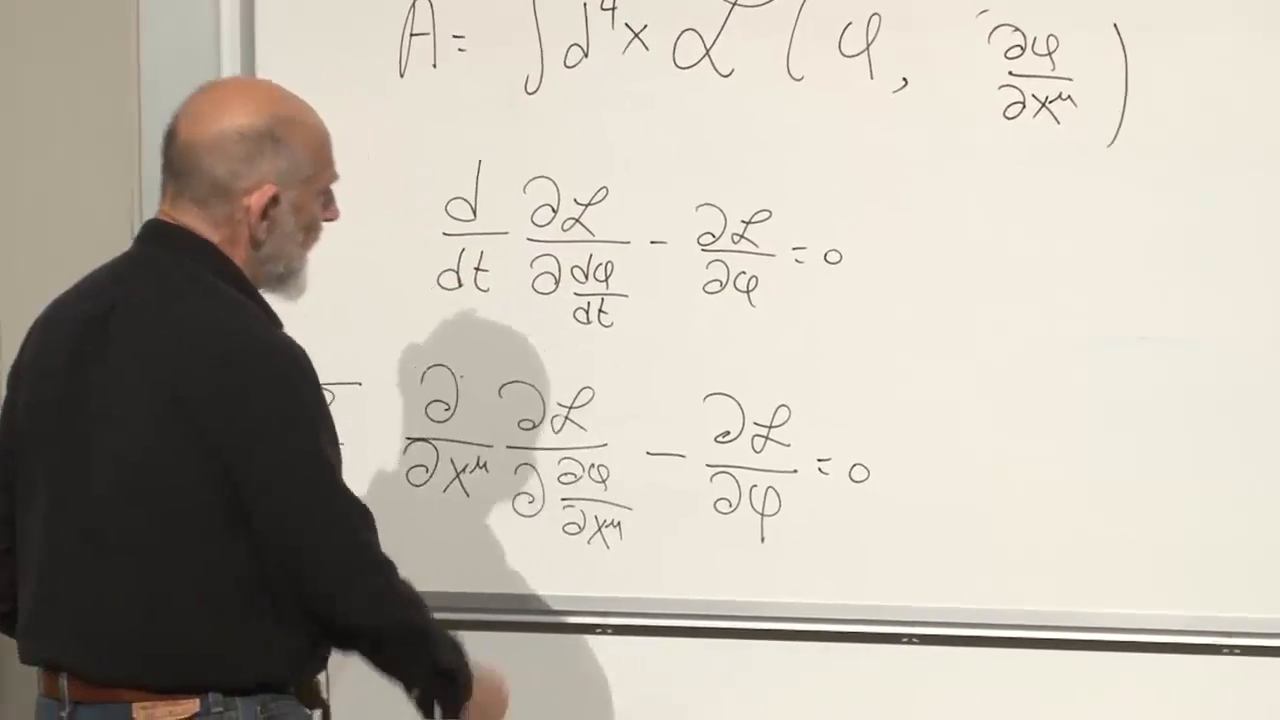
\includegraphics[width=0.90\textwidth]{lecture_04_figure_05.png}\caption{Die Wirkungsdichte als lokale Funktion von \(\phi\) und seinen Raumzeit-Ableitungen.}\lectureframe{00:32:51}\end{figure}

\begin{classroomqa}\audiencequestion{Kann die Lagrange-Dichte auch von \(x,y,z\) selbst abhängen?}\lecturerresponse{Das ist möglich, ebenso wie eine Teilchen-Lagrange-Funktion explizit von \(t\) abhängen kann. Bei einem translationsinvarianten abgeschlossenen System ist das üblicherweise nicht der Fall, aber eine explizite Koordinatenabhängigkeit macht die Formulierung nicht ungültig. \lecturetimestamp{00:30:29}}\end{classroomqa}

\begin{classroomqa}\audiencequestion{Gilt die bisherige Konstruktion speziell für ein Skalarfeld oder ist sie allgemein?}\lecturerresponse{Das Variationsschema ist bisher allgemein. Dass nur eine Komponente geschrieben wird, deutet auf ein Skalarfeld hin. Ein Vektorfeld oder eine Sammlung von Feldern hätte zusätzliche Komponentenindizes, und jede Komponente würde variiert. \lecturetimestamp{00:31:00}}\end{classroomqa}

\subsection{Das Gitterbild}

Auf einem feinen Raumzeitgitter werden Ableitungen zu Differenzen zwischen benachbarten Feldwerten. Die Wirkung ist dann eine gewöhnliche Funktion vieler Variablen. Ein Gitter mit zehn Punkten in der einen und acht in der anderen Richtung hat bereits achtzig Feldvariablen. Bei einer Verfeinerung des Gitters nimmt ihre Zahl zu, aber die Minimierungsregel bleibt einfach: Man leitet die Wirkung nach dem Feldwert an jedem inneren Punkt ab und setzt das Ergebnis gleich null.

\begin{figure}[htbp]\centering
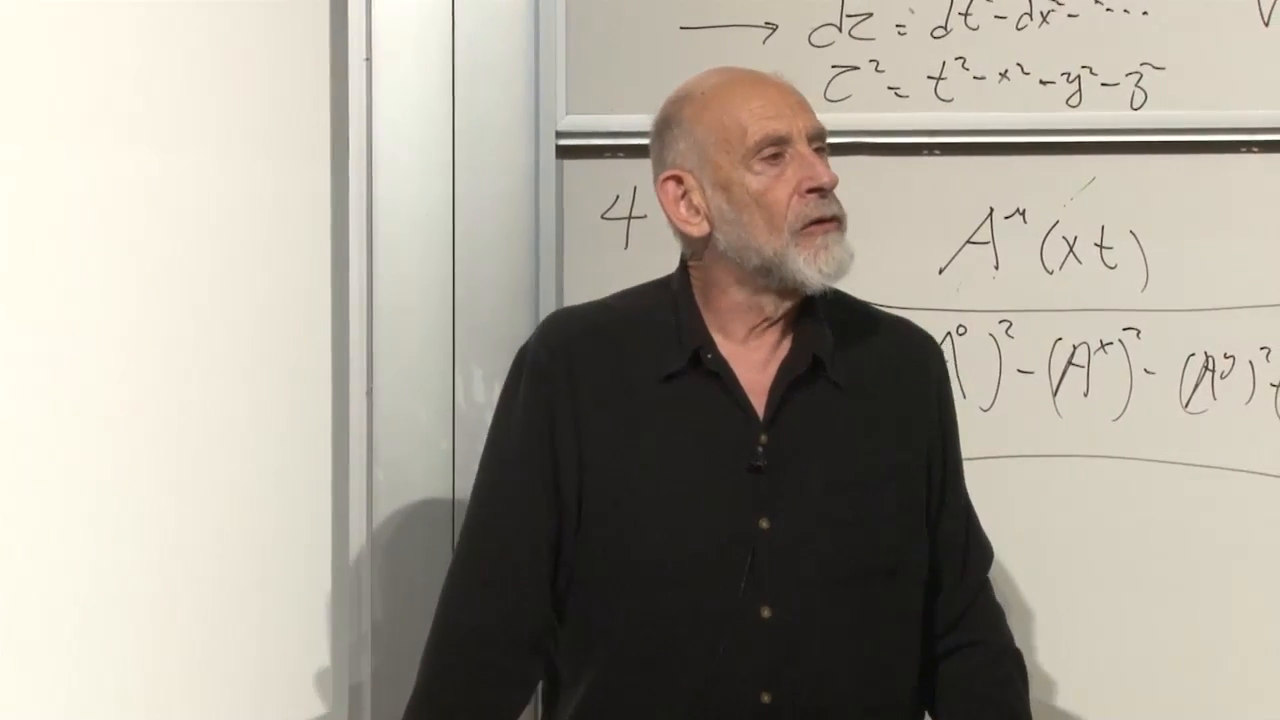
\includegraphics[width=0.90\textwidth]{lecture_04_figure_06.png}\caption{Das in Zellen unterteilte Raumzeitgebiet: Vor dem Kontinuumslimes wird die Wirkung so zu einer gewöhnlichen Funktion vieler Variablen.}\lectureframe{00:34:05}\end{figure}

Im Kontinuumslimes erhält man die Euler--Lagrange-Gleichung des Feldes, \begin{equation}
\boxed{
\partial_\mu
\left[
\frac{\partial\mathcal{L}}
{\partial(\partial_\mu\phi)}
\right]
-
\frac{\partial\mathcal{L}}{\partial\phi}
=0
}.
\label{eq:sr4-field-el}
\end{equation} Über den wiederholten Index \(\mu\) wird über alle Raumzeitrichtungen summiert. Ohne diese Summationskonvention lautet dieselbe Gleichung \begin{align}
&
\frac{\partial}{\partial t}
\left(\frac{\partial\mathcal{L}}{\partial\phi_t}\right)
+
\frac{\partial}{\partial x}
\left(\frac{\partial\mathcal{L}}{\partial\phi_x}\right)
+
\frac{\partial}{\partial y}
\left(\frac{\partial\mathcal{L}}{\partial\phi_y}\right)
\nonumber\\
&\hspace{3em}
+
\frac{\partial}{\partial z}
\left(\frac{\partial\mathcal{L}}{\partial\phi_z}\right)
-
\frac{\partial\mathcal{L}}{\partial\phi}
=0.
\label{eq:sr4-field-el-expanded}
\end{align} Der erste Term ist aus der Teilchenmechanik vertraut. Die Feldtheorie ergänzt einen analogen Term für jede räumliche Richtung. Der letzte Term, \(-\partial\mathcal{L}/\partial\phi\), bleibt unverändert.

\begin{figure}[htbp]\centering
\includegraphics[width=0.90\textwidth]{lecture_04_figure_07.png}\caption{Die eindimensionale Euler--Lagrange-Gleichung und ihre Raumzeitverallgemeinerung, untereinander dargestellt.}\lectureframe{00:38:44}\end{figure}

Dieses Gebiet wird auch Kontinuumsmechanik genannt. Je nach den Freiheitsgraden kann dieselbe Mathematik Strömungen, elastische Verformungen oder ein anderes kontinuierliches Medium beschreiben.

\begin{classroomqa}\audiencequestion{Würden dieselben Gleichungen in einer Welt mit Raum, aber ohne Zeit funktionieren?}\lecturerresponse{Ja, als rein räumliches Variationsproblem. Physikalisch sucht man so nach einer statischen Lösung: Man nimmt an, dass das Feld zeitunabhängig ist, verwirft alle Zeitableitungen und löst die verbleibenden räumlichen Gleichungen. Eine zeitunabhängige elektrische oder magnetische Konfiguration ist ein Beispiel. \lecturetimestamp{00:40:05}}\end{classroomqa}

\section{Die einfachste Skalarfelddynamik erschließen}

\subsection{Warum die Vorzeichen nicht alle gleich sein können}

Kehren wir zum kinetischen Term des Teilchens \(\tfrac12\dot\phi^2\) zurück, setzen wir seinen irrelevanten Gesamtfaktor auf eins und versuchen wir, ihn zu verallgemeinern. Ein erster Ansatz könnte \begin{equation}
\mathcal{L}_{+}
=
\frac12
\left[
\phi_t^2+\phi_x^2+\phi_y^2+\phi_z^2
\right].
\label{eq:sr4-all-plus}
\end{equation} sein. Das ist ein nützlicher Irrweg. Er behandelt Zeit und Raum mit gleichen Vorzeichen. Die resultierende Gleichung hätte nicht die hyperbolische Struktur der Wellenausbreitung. Die korrekte relativistische Kombination hat für die Zeit ein Vorzeichen und für den Raum das entgegengesetzte.

\begin{classroomqa}\audiencequestion{Ist der Ausdruck mit ausschließlich positiven Vorzeichen falsch, weil die Lagrange-Funktion relativistisch invariant sein muss?}\lecturerresponse{Das ist die grundlegendere Antwort, und sie ist richtig. Die Vorlesung gelangt zunächst auf anschaulichere Weise zu den Vorzeichen: Wellen unterscheiden die zeitliche Entwicklung von der räumlichen Variation, daher darf die Zeit nicht genau wie eine weitere räumliche Koordinate eingehen. Die Lorentz-Invarianz wird diese Anschauung gleich in eine präzise Regel überführen. \lecturetimestamp{00:43:19}}\end{classroomqa}

Stellen wir eine charakteristische Geschwindigkeit \(c\) wieder her, so lautet die einfache Lagrange-Dichte des Skalarfeldes \begin{equation}
\boxed{
\mathcal{L}
=
\frac12
\left[
\frac{1}{c^2}\phi_t^2
-\phi_x^2-\phi_y^2-\phi_z^2
\right]
-V(\phi)
}.
\label{eq:sr4-scalar-lagrangian}
\end{equation} Für ein relativistisches Feld ist \(c\) die Lichtgeschwindigkeit. In einem Kontinuumsmodell könnte es stattdessen die Schallgeschwindigkeit, die Geschwindigkeit einer elastischen Welle oder eine andere charakteristische Ausbreitungsgeschwindigkeit sein.

Der Gesamtfaktor \(1/2\) ist Konvention, genauso wie bei \(\tfrac12m\dot\phi^2\). Multipliziert man eine gesamte Wirkung mit einer von null verschiedenen Konstanten, ändern sich ihre stationären Pfade nicht; die Konvention legt fest, wie die Parameter in den Gleichungen benannt und normiert werden. Ist diese Normierung einmal gewählt, muss sie konsequent verwendet werden.

\begin{classroomqa}\audiencequestion{Kann man die Terme mit räumlichen Gradienten als Teil der potenziellen Energie auffassen?}\lecturerresponse{Ja. Bei der Aufteilung in kinetische minus potenzielle Energie enthält der kinetische Anteil Zeitableitungen. Terme ohne Zeitableitungen, darunter räumliche Gradienten und \(V(\phi)\), gehören zum Anteil der potenziellen Energie. Der letztliche Grund für ihre relativen Vorzeichen in einer relativistischen Theorie ist die Lorentz-Metrik. \lecturetimestamp{00:45:37}}\end{classroomqa}

\subsection{Die Wellengleichung}

Wenden wir \eqref{eq:sr4-field-el} an. Für die Ableitungsterme gilt \begin{equation}
\frac{\partial\mathcal{L}}{\partial\phi_t}
=\frac{1}{c^2}\phi_t,
\qquad
\frac{\partial\mathcal{L}}{\partial\phi_i}
=-\phi_i,
\end{equation} während \begin{equation}
\frac{\partial\mathcal{L}}{\partial\phi}
=-\frac{dV}{d\phi}.
\end{equation} Damit folgt \begin{equation}
\begin{aligned}
&\boxed{
\frac{1}{c^2}\frac{\partial^2\phi}{\partial t^2}
-\nabla^2\phi
+\frac{dV}{d\phi}
=0
},\\[0.5em]
\nabla^2
&=
\frac{\partial^2}{\partial x^2}
+\frac{\partial^2}{\partial y^2}\\
&\quad
+\frac{\partial^2}{\partial z^2}.
\end{aligned}
\label{eq:sr4-general-scalar-eom}
\end{equation}

Für \(V=0\) vereinfacht sich dies zu \begin{equation}
\boxed{
\frac{1}{c^2}\phi_{tt}-\nabla^2\phi=0
},
\label{eq:sr4-wave-equation}
\end{equation} der Wellengleichung. Die Vorlesung erkennt die Gleichung, verschiebt ihre Lösung aber auf später. Ihre Lösungen breiten Störungen mit der Geschwindigkeit \(c\) aus.

\begin{figure}[htbp]\centering
\includegraphics[width=0.90\textwidth]{lecture_04_figure_08.png}\caption{Die eindimensionale Form \(c^{-2}\phi_{tt}-\phi_{xx}=0\), erkannt als Wellengleichung.}\lectureframe{00:50:30}\end{figure}

\subsection{Ein Feld gekoppelter harmonischer Oszillatoren}

Wählen wir nun ein quadratisches Potential, \begin{equation}
V(\phi)=\frac12\mu^2\phi^2,
\qquad
\frac{dV}{d\phi}=\mu^2\phi.
\label{eq:sr4-quadratic-potential}
\end{equation} Wäre \(\phi\) die Position eines Teilchens, so wäre dies das Potential eines harmonischen Oszillators mit der Federkonstante \(\mu^2\). Für das Feld gilt \begin{equation}
\boxed{
\frac{1}{c^2}\phi_{tt}-\nabla^2\phi+\mu^2\phi=0
}.
\label{eq:sr4-klein-gordon}
\end{equation} Ohne die räumliche Ableitung ist dies einfach eine Beschleunigung plus eine Konstante mal Auslenkung, gleich null. Der Gradient koppelt benachbarte Punkte und macht aus dem Oszillator ein wellentragendes Kontinuum. In der relativistischen Feldtheorie heißt \eqref{eq:sr4-klein-gordon} massive Klein--Gordon-Gleichung; klassisch ist \(\mu\) die inverse Längenskala, die die Wellenausbreitung verändert.

\begin{figure}[htbp]\centering
\includegraphics[width=0.90\textwidth]{lecture_04_figure_09.png}\caption{Das quadratische Potential und die daraus folgende Wellengleichung mit dem Rückstellterm \(\mu^2\phi\).}\lectureframe{00:52:38}\end{figure}

\begin{classroomqa}\audiencequestion{Warum verschwindet der Faktor \(1/2\) in \(V=\tfrac12\mu^2\phi^2\) aus der Bewegungsgleichung?}\lecturerresponse{Beim Ableiten von \(\phi^2\) entsteht ein Faktor zwei. Der konventionelle Faktor \(1/2\) wird genau deshalb eingeführt, damit \(dV/d\phi=\mu^2\phi\) gilt, so wie \(V(x)=\tfrac12kx^2\) die Rückstellkraft \(-kx\) ergibt. \lecturetimestamp{00:53:17}}\end{classroomqa}

Die Gleichung ist linear: \(\phi\) und jede seiner Ableitungen treten nur in erster Potenz auf. Terme wie \(\phi^2\) oder \(\phi\,\partial_\mu\phi\) in der Bewegungsgleichung würden die Dynamik nichtlinear machen.

\section{Lorentz-Skalare und Vierervektoren}

\subsection{Die Wirkung muss bezugssystemunabhängig sein}

Die Variationsmethodik allein legt viele mögliche Feldtheorien fest. Die Relativitätstheorie stellt zusätzlich die Forderung, dass die Wirkung in jedem Inertialsystem denselben Wert und dieselbe Form hat. Beim freien Teilchen wurde dies erreicht, indem man die invariante Eigenzeit \(d\tau\) entlang der Weltlinie integrierte. Bei einem Feld wird die Wirkung über die Raumzeit integriert; daher müssen sich ihre lokalen Bausteine in geeigneter Weise transformieren.

Unter einer eigentlichen Lorentz-Transformation ist das Raumzeitmaß invariant, \(d^4x'=d^4x\). Daher genügt es, von der Lagrange-Dichte zu verlangen, dass sie ein Lorentz-Skalar ist: \begin{equation}
\mathcal{L}'(x')=\mathcal{L}(x).
\label{eq:sr4-lagrangian-scalar}
\end{equation}

\subsection{Skalarfelder}

Ein Skalarfeld erfüllt \begin{equation}
\boxed{\phi'(x')=\phi(x)}.
\label{eq:sr4-scalar-transform}
\end{equation} Die Koordinaten \(x\) und \(x'\) bezeichnen dasselbe Ereignis in zwei Bezugssystemen. Die von den Beobachtern verwendeten Funktionsterme können unterschiedlich aussehen, aber der diesem physikalischen Ereignis zugeordnete Zahlenwert ist derselbe.

\begin{figure}[htbp]\centering
\includegraphics[width=0.90\textwidth]{lecture_04_figure_10.png}\caption{Das definierende Transformationsgesetz eines Skalarfeldes: \(\phi(x)=\phi'(x')\).}\lectureframe{00:59:33}\end{figure}

Die Temperatur lieferte die erste Anschauung, auch wenn ein bewegtes Thermometer in einem materiellen Medium kein vollkommenes relativistisches Beispiel ist. Entscheidend ist die Definition \eqref{eq:sr4-scalar-transform}, nicht die Analogie mit dem Thermometer.

\subsection{Vierervektoren}

In Einheiten \(c=1\) wirkt ein Boost mit der Geschwindigkeit \(v\) entlang der \(x\)-Achse wie folgt: \begin{equation}
\begin{aligned}
t'&=\gamma(t-vx),\\
x'&=\gamma(x-vt),\\
y'&=y,\\
z'&=z,\\
\gamma&=\frac{1}{\sqrt{1-v^2}}.
\end{aligned}
\label{eq:sr4-x-boost}
\end{equation}

\begin{figure}[htbp]\centering
\includegraphics[width=0.90\textwidth]{lecture_04_figure_11.png}\caption{Die Lorentz-Transformation für einen Boost entlang der \(x\)-Achse in Einheiten \(c=1\).}\lectureframe{01:02:26}\end{figure}

Vier Größen, die sich unter Boosts auf dieselbe Weise mischen, bilden einen Vierervektor. Beispiele, denen wir bereits begegnet sind, sind \(x^\mu\), \(dx^\mu\) und die Vierergeschwindigkeit \(u^\mu=dx^\mu/d\tau\). Das Produkt eines Vierervektors mit einem Skalar ergibt wieder einen Vierervektor. Eine strömende relativistische Flüssigkeit liefert ein feldwertiges Beispiel: Ihre Vierergeschwindigkeit \(u^\mu(x)\) kann sich von Ereignis zu Ereignis unterscheiden.

Für denselben Boost wie in \eqref{eq:sr4-x-boost} erfüllt ein allgemeiner Vierervektor \begin{equation}
\begin{aligned}
A'^0&=\gamma(A^0-vA^x),\\
A'^x&=\gamma(A^x-vA^0),\\
A'^y&=A^y,\\
A'^z&=A^z.
\end{aligned}
\label{eq:sr4-vector-boost}
\end{equation}

Für einen allgemeinen Vierervektor \(A^\mu=(A^0,A^x,A^y,A^z)\) ist die Lorentzsche Norm \begin{equation}
\boxed{
A_\mu A^\mu
=(A^0)^2-(A^x)^2-(A^y)^2-(A^z)^2
}
\label{eq:sr4-vector-norm}
\end{equation} ein Skalar. Sie ist aus demselben algebraischen Grund invariant wie \begin{equation}
d\tau^2=dt^2-dx^2-dy^2-dz^2
\end{equation}. Der Vorlesung gehen kurz die unverbrauchten Buchstaben für einen allgemeinen Vektor aus, bevor sie \(A\) akzeptiert, angeregt durch den Vorschlag \(A\) als Abkürzung für „arrow“ zu verwenden.

\begin{figure}[htbp]\centering
\includegraphics[width=0.90\textwidth]{lecture_04_figure_12.png}\caption{Ein allgemeines Vierervektorfeld und die Lorentzsche Differenz der Quadrate, aus der seine invariante Norm gebildet wird.}\lectureframe{01:09:06}\end{figure}

\subsection{Die Ableitung eines Skalarfeldes}

Die Ableitung eines Skalarfeldes nach den vier Raumzeitkoordinaten ergibt die vier Komponenten \begin{equation}
\partial_\mu\phi
=
\left(
\frac{\partial\phi}{\partial t},
\frac{\partial\phi}{\partial x},
\frac{\partial\phi}{\partial y},
\frac{\partial\phi}{\partial z}
\right)
\qquad(c=1).
\end{equation} Streng genommen ist \(\partial_\mu\phi\) eine Kovektorkomponente; durch Anheben des Index mit der Minkowski-Metrik erhält man \(\partial^\mu\phi\). Für das Komponentenargument hier ist dieser Unterschied unerheblich, doch er legt die Kontraktion eindeutig fest: \begin{equation}
\boxed{
\partial_\mu\phi\,\partial^\mu\phi
=
\frac{1}{c^2}\phi_t^2
-\phi_x^2-\phi_y^2-\phi_z^2
}.
\label{eq:sr4-derivative-scalar}
\end{equation}

\begin{figure}[htbp]\centering
\includegraphics[width=0.90\textwidth]{lecture_04_figure_13.png}\caption{Die invariante Differenz der Quadrate aus den ersten Ableitungen eines Skalarfeldes.}\lectureframe{01:13:55}\end{figure}

\begin{classroomqa}\audiencequestion{Ist diese Kombination von Ableitungen der Laplace-Operator?}\lecturerresponse{Nein. Die dargestellte invariante Größe ist quadratisch in den ersten Ableitungen. Der Laplace-Operator enthält zweite räumliche Ableitungen. Zweite Ableitungen treten erst nach der Variation der Wirkung in der Wellengleichung auf. \lecturetimestamp{01:13:22}}\end{classroomqa}

Das Vorzeichenmuster in \eqref{eq:sr4-scalar-lagrangian} lässt sich jetzt erklären, statt es nur zu erraten. Die Kombination aus kinetischem Term und Gradient ist der Lorentz-Skalar \(\partial_\mu\phi\,\partial^\mu\phi\). Damit lautet die einfachste quadratische Theorie \begin{equation}
\mathcal{L}
=
\frac12\partial_\mu\phi\,\partial^\mu\phi
-\frac12\mu^2\phi^2.
\label{eq:sr4-covariant-lagrangian}
\end{equation}

\begin{figure}[htbp]\centering
\includegraphics[width=0.90\textwidth]{lecture_04_figure_14.png}\caption{Die vervollständigte quadratische Lagrange-Dichte des Skalarfeldes und ihre lineare Feldgleichung an der Tafel.}\lectureframe{01:19:12}\end{figure}

\section{Wie viel Freiheit gibt es?}

Sobald die Regel zur Bildung von Skalaren bekannt ist, sind viele Lagrange-Dichten möglich. Das Feld \(\phi\) ist ein Skalar, also ist auch jede gewöhnliche Funktion \(F(\phi)\) ein Skalar: \(\phi^2\), \(\phi^3\), \(\cosh\phi\) und so weiter. Auch numerische Parameter sind zulässig. Ein Symbol wie \(\mu\) kann als konstanter Koeffizient eingesetzt werden; offen bleiben nur seine Dimensionen und seine physikalische Deutung.

\begin{classroomqa}\audiencequestion{Kann man eine Masse in die Lagrange-Dichte aufnehmen?}\lecturerresponse{Ein konstanter Parameter ist gewiss zulässig. An dieser Stelle sollte man fragen, um die Masse welchen Objekts es sich handelt, denn \(\mu\) ist in der klassischen Feldtheorie zunächst einfach eine Zahl, bis ihre physikalische Bedeutung bestimmt ist. In der quadratischen relativistischen Skalarfeldtheorie legt sie die Masse oder die inverse Längenskala fest. \lecturetimestamp{01:14:16}}\end{classroomqa}

Skalare lassen sich miteinander multiplizieren: \begin{equation}
F(\phi)\,\partial_\mu\phi\,\partial^\mu\phi
\end{equation} ist Lorentz-invariant. Auch der Ableitungsskalar selbst kann quadriert werden, wodurch höhere Potenzen erster Ableitungen entstehen. Ebenso kann man höhere Ableitungen in Betracht ziehen, doch die Vorlesung beschränkt sich auf Felder und ihre ersten Ableitungen, den üblichen Rahmen, der Bewegungsgleichungen zweiter Ordnung liefert. Bei Theorien mit höheren Ableitungen ist zusätzliche Sorgfalt nötig, weil sie im Allgemeinen weitere dynamische Daten und mögliche Instabilitäten mit sich bringen.

\begin{classroomqa}\audiencequestion{Ist die Konstruktion als Differenz von Quadraten tatsächlich die Metrik der Raumzeit?}\lecturerresponse{Ja. In der gewählten Signatur lautet die Metrik \(dt^2-dx^2-dy^2-dz^2\). Das Wort „Metrik“ wurde in der Vorlesung bisher nicht hervorgehoben, aber genau diese Raumzeitgeometrie wird in der allgemeinen Relativitätstheorie zentral werden. \lecturetimestamp{01:19:39}}\end{classroomqa}

\begin{classroomqa}\audiencequestion{Gibt es allgemeinere Objekte als Vierervektoren mit Komponenten wie \(xy\) oder \(tx\)?}\lecturerresponse{Ja. Das sind Tensoren. Ein Skalar hat keinen Raumzeitindex, ein Vektor einen und ein Tensor zweiten Ranges Komponenten wie \(T^{xx}\), \(T^{xy}\) und \(T^{tx}\). Der größte Teil der bisherigen Diskussion über Skalarfelder kommt ohne sie aus; in der allgemeinen Relativitätstheorie sind sie unverzichtbar. \lecturetimestamp{01:20:49}}\end{classroomqa}

\begin{classroomqa}\audiencequestion{Warum betrachtet man nur Boosts, die \(t\) mit \(x\) mischen? Könnte ein Boost in eine andere Richtung zeigen und die Raumachsen anders mischen?}\lecturerresponse{Durchaus. Ein Boost entlang \(y\) mischt \(t\) mit \(y\) und lässt \(x,z\) unverändert. Eine allgemeine Lorentz-Transformation lässt sich aus räumlichen Drehungen und einem Boost entlang einer gewählten Achse zusammensetzen. Es genügt daher, die Rotationsinvarianz und die Invarianz unter einem Boost entlang einer Standardachse nachzuweisen. \lecturetimestamp{01:22:06}}\end{classroomqa}

\begin{classroomqa}\audiencequestion{Beschreiben alle Lagrange-Dichten, die sich aus so vielen möglichen Skalarmischungen ergeben, sinnvolle Physik?}\lecturerresponse{Auf klassischer Ebene ist die Freiheit enorm, sofern zusätzliche Anforderungen wie sinnvolle Vorzeichen, Lokalität und ein wohldefiniertes Evolutionsproblem erfüllt sind. Deutlich weniger willkürliche Wahlmöglichkeiten ergeben wohldefinierte fundamentale Quantentheorien. Die moderne effektive Feldtheorie lässt viele weitere Wechselwirkungen unterhalb einer Abschneideskala zu; dann muss jedoch der Gültigkeitsbereich angegeben werden. \lecturetimestamp{01:27:57}}\end{classroomqa}

\begin{classroomqa}\audiencequestion{Muss ein Feld stetig sein?}\lecturerresponse{Für die hier betrachteten glatten Theorien: ja. Ein Sprung führt zu singulären Ableitungen und bei einem quadratischen Gradiententerm typischerweise zu unendlicher Wirkung und Energie. Singulärere Konfigurationen lassen sich nur mit zusätzlicher mathematischer Struktur behandeln; sie sind nicht die gewöhnlichen Felder endlicher Energie, die hier entwickelt werden. \lecturetimestamp{01:29:29}}\end{classroomqa}

\section{Ein Teilchen in Kopplung an ein Skalarfeld}

\subsection{Das freie Teilchen erneut betrachtet}

Im letzten Teil der Vorlesung werden Teilchen und Felder auf klassischer Ebene zusammengeführt. Es geht noch nicht um die quantenmechanische Aussage, dass Teilchen Anregungen von Feldern sind. Nehmen wir stattdessen an, jemand habe bereits ein Hintergrund-Skalarfeld \(\phi(x,t)\) berechnet, und fragen wir, wie sich ein Teilchen darin bewegt.

Für ein freies relativistisches Teilchen gilt
\begin{equation}
A_{\rm free}=-m\int d\tau.
\label{eq:sr4-free-particle-action}
\end{equation}
In einer Raumdimension und bei \(c=1\) gilt
\begin{equation}
d\tau=dt\sqrt{1-\dot x^2},
\qquad
L_{\rm free}=-m\sqrt{1-\dot x^2}.
\label{eq:sr4-free-particle-l}
\end{equation}
Das Minuszeichen wird so gewählt, dass die Entwicklung für kleine Geschwindigkeiten den üblichen positiven Newtonschen kinetischen Term ergibt:
\begin{equation}
L_{\rm free}
\approx -m+\frac12m\dot x^2+\cdots.
\end{equation}

\begin{figure}[htbp]
\centering
\includegraphics[width=0.90\textwidth]{lecture_04_figure_15.png}
\caption{Die invariante Wirkung für ein freies Teilchen, umgeschrieben als Lagrange-Funktion bezüglich der Koordinatenzeit.}
\lectureframe{01:34:31}
\end{figure}

\subsection{Die einfachste skalare Kopplung}

Sowohl \(d\tau\) als auch \(\phi\) sind Skalare. Die einfachste lineare Kopplung lautet daher
\begin{equation}
\boxed{
A
=
\int d\tau\,[-m+\phi(x,t)]
}.
\label{eq:sr4-coupled-action}
\end{equation}
Diese Wahl ist nicht eindeutig. Man könnte \(\phi\) durch eine beliebige Funktion \(F(\phi)\) ersetzen. Der lineare Term genügt, um die physikalische Idee zu veranschaulichen.

\begin{figure}[htbp]
\centering
\includegraphics[width=0.90\textwidth]{lecture_04_figure_16.png}
\caption{Die freie Wirkung ergänzt um die einfachste Lorentz-invariante skalare Kopplung.}
\lectureframe{01:37:21}
\end{figure}

\begin{classroomqa}
\audiencequestion{Muss \(\phi\) innerhalb des Integrals bleiben?}
\lecturerresponse{Ja. Das Feld wird auf der Weltlinie des Teilchens ausgewertet, \(\phi(x(t),t)\), und ändert sich im Allgemeinen von einem Punkt der Bahn zum nächsten. Selbst wenn der Hintergrund keine explizite Zeitabhängigkeit aufweist, \(\phi=\phi(x)\), ändert er sich dennoch mit der Zeit, wenn sich das Teilchen durch den Raum bewegt. Nur ein entlang der Bahn konstantes Feld könnte vor das Integral gezogen werden. \lecturetimestamp{01:37:47}}
\end{classroomqa}

\begin{classroomqa}
\audiencequestion{Bedeutet das \(x\) in \(\phi(x,t)\) die Position des Teilchens?}
\lecturerresponse{Ja. Es ist \(x=x(t)\), die Position des Teilchens zum Zeitpunkt \(t\). Die Wirkung erfasst das vorgegebene Raumzeitfeld entlang dieser Bahn. \lecturetimestamp{01:38:08}}
\end{classroomqa}

Für eine eindimensionale Bewegung ergibt sich aus \eqref{eq:sr4-coupled-action}
\begin{equation}
L
=
-(m-\phi(x,t))\sqrt{1-\dot x^2}.
\label{eq:sr4-coupled-lagrangian}
\end{equation}
Das skalare Hintergrundfeld tritt genau an die Stelle der Ruhemasse:
\begin{equation}
m_{\rm eff}(x,t)=m-\phi(x,t).
\label{eq:sr4-effective-mass}
\end{equation}
Wenn sich \(\phi\) auf einen nahezu konstanten, von null verschiedenen Wert einpendelt, verhält sich das Teilchen, als hätte sich seine Masse geändert. Dies ist nur ein klassisches Spielzeugmodell und nicht der vollständige Higgs-Mechanismus, vermittelt aber einen Eindruck von der Grundidee des Higgs-Mechanismus: Ein skalarer Hintergrund kann als Massenterm in die Teilchendynamik eingehen.

\subsection{Die Teilchengleichung}

Der kanonische Impuls lautet
\begin{equation}
p
=
\frac{\partial L}{\partial\dot x}
=
(m-\phi)
\frac{\dot x}{\sqrt{1-\dot x^2}}.
\label{eq:sr4-coupled-momentum}
\end{equation}

\begin{figure}[htbp]
\centering
\includegraphics[width=0.90\textwidth]{lecture_04_figure_17.png}
\caption{Der skalare Hintergrund ersetzt \(m\) durch \(m-\phi(x,t)\) im relativistischen kanonischen Impuls.}
\lectureframe{01:43:38}
\end{figure}

Die Ortsableitung der Lagrange-Funktion lautet
\begin{equation}
\frac{\partial L}{\partial x}
=
\frac{\partial\phi}{\partial x}
\sqrt{1-\dot x^2}.
\end{equation}
Bei festgehaltenem Vorzeichen, das durch die Wirkung \eqref{eq:sr4-coupled-action} vorgegeben ist, lautet die Euler--Lagrange-Gleichung daher
\begin{equation}
\boxed{
\frac{d}{dt}
\left[
(m-\phi)
\frac{\dot x}{\sqrt{1-\dot x^2}}
\right]
=
\frac{\partial\phi}{\partial x}
\sqrt{1-\dot x^2}
}.
\label{eq:sr4-coupled-eom}
\end{equation}

\begin{figure}[htbp]
\centering
\includegraphics[width=0.90\textwidth]{lecture_04_figure_18.png}
\caption{Die gekoppelte Gleichung wird aus dem Impuls und der räumlichen Ableitung des Hintergrundfeldes zusammengesetzt; die Wirkung legt das endgültige Vorzeichen in \eqref{eq:sr4-coupled-eom} fest.}
\lectureframe{01:45:24}
\end{figure}

\begin{classroomqa}
\audiencequestion{Warum bleibt in \(\partial\phi/\partial x\) der Faktor \(\sqrt{1-\dot x^2}\) erhalten?}
\lecturerresponse{Weil nur der Faktor \(\phi(x,t)\) nach \(x\) abgeleitet wird. In der Lagrange-Funktion wird er mit der Quadratwurzel multipliziert, die bei festgehaltenem \(\dot x\) in der partiellen Ableitung nicht von der Position abhängt. Daher bleibt die Quadratwurzel erhalten. \lecturetimestamp{01:45:50}}
\end{classroomqa}

Durch Ausmultiplizieren der totalen Zeitableitung ergibt sich
\begin{align}
&(m-\phi)
\frac{d}{dt}
\left(
\frac{\dot x}{\sqrt{1-\dot x^2}}
\right)
-
\dot\phi\,
\frac{\dot x}{\sqrt{1-\dot x^2}}
\nonumber\\
&\hspace{10em}
=
\frac{\partial\phi}{\partial x}
\sqrt{1-\dot x^2}.
\label{eq:sr4-coupled-expanded}
\end{align}
Ist der Hintergrund statisch, \(\phi=\phi(x)\), ist seine Ableitung entlang der bewegten Weltlinie nicht null. Die Kettenregel ergibt
\begin{equation}
\boxed{
\dot\phi
=
\frac{d}{dt}\phi(x(t))
=
\frac{\partial\phi}{\partial x}\dot x
}.
\label{eq:sr4-chain-rule}
\end{equation}

\begin{classroomqa}
\audiencequestion{Wenn \(\phi\) keine explizite Zeitabhängigkeit hat, warum ist \(\dot\phi\) nicht null?}
\lecturerresponse{Weil das Teilchen seine Position ändert. Das Feld wird bei \(x(t)\) ausgewertet, daher lautet seine totale Ableitung \(\dot\phi=\phi_x\dot x\). Ein statisches Feld bedeutet \(\partial\phi/\partial t=0\), nicht, dass jedes bewegte Teilchen einen konstanten Feldwert erfährt. \lecturetimestamp{01:48:10}}
\end{classroomqa}

\begin{figure}[htbp]
\centering
\includegraphics[width=0.90\textwidth]{lecture_04_figure_19.png}
\caption{Die Entwicklung der gekoppelten Gleichung nach Anwendung der Kettenregel entlang der Weltlinie.}
\lectureframe{01:49:11}
\end{figure}

Der exakte Ausdruck ist nicht besonders elegant, und die Vorlesung behauptet auch nicht, dass er es wäre. Der Grenzfall kleiner Geschwindigkeiten ist dennoch vertraut. Da \(\sqrt{1-\dot x^2}\approx1\), lautet die führende Gleichung
\begin{equation}
\frac{d}{dt}\bigl[(m-\phi)\dot x\bigr]
\approx
\frac{\partial\phi}{\partial x}.
\end{equation}
Wird auch die Variation der effektiven Masse störungstheoretisch behandelt, vereinfacht sich dies zu
\begin{equation}
(m-\phi)\ddot x
\approx
\frac{\partial\phi}{\partial x}.
\label{eq:sr4-nonrel-force}
\end{equation}
Tatsächlich lautet die Lagrange-Funktion bei kleinen Geschwindigkeiten
\begin{equation}
L
\approx
-m+\phi+\frac12(m-\phi)\dot x^2,
\end{equation}
Somit sind in führender Ordnung die potenzielle Energie \(U=-\phi\) und die Kraft \(-dU/dx=\partial_x\phi\). Die Faktoren \(c\) wieder einzusetzen und dieses Newtonsche Muster wiederzugewinnen, ist die Aufgabe, mit der die Vorlesung endet.

Der Weg von Teilchen zu Feldern ist nun abgeschlossen. Eine Teilchengeschichte \(\phi(t)\) lieferte das \(0+1\)-dimensionale Grundmodell; eine Feldgeschichte \(\phi(x)\) erweiterte die Wirkung zu einem Raumzeitintegral; die Feld-Euler--Lagrange-Gleichung führte zur Wellendynamik; Lorentz-Skalare legten die relativistische Vorzeichenstruktur fest; und dieselbe Invariantensprache ermöglichte es einem skalaren Hintergrund, auf ein Teilchen zurückzuwirken.
